\documentclass{article}
\usepackage[utf8]{inputenc}
\usepackage{xcolor}
\usepackage{polski}
% Default fixed font does not support bold face
\DeclareFixedFont{\ttb}{T1}{txtt}{bx}{n}{12} % for bold
\DeclareFixedFont{\ttm}{T1}{txtt}{m}{n}{12}  % for normal

% Custom colors
\usepackage{color}
\definecolor{deepblue}{rgb}{0,0,0.5}
\definecolor{deepred}{rgb}{0.6,0,0}
\definecolor{deepgreen}{rgb}{0,0.5,0}

\usepackage{listings}

% Python style for highlighting
\newcommand\pythonstyle{\lstset{
language=Python,
basicstyle=\ttm,
otherkeywords={self},             % Add keywords here
keywordstyle=\ttb\color{deepblue},
emph={MyClass,__init__},          % Custom highlighting
emphstyle=\ttb\color{deepred},    % Custom highlighting style
stringstyle=\color{deepgreen},
frame=tb,                         % Any extra options here
showstringspaces=false            % 
}}


% Python environment
\lstnewenvironment{python}[1][]
{
\pythonstyle
\lstset{#1}
}
{}

% Python for external files
\newcommand\pythonexternal[2][]{{
\pythonstyle
\lstinputlisting[#1]{#2}}}

% Python for inline
\newcommand\pythoninline[1]{{\pythonstyle\lstinline!#1!}}

\author   {Dominika Pienczyn}
\title    {Porównanie klasyfikatorów na wybranej bazie danych}
\date     {2020}

\usepackage{natbib}
\usepackage{graphicx}
\usepackage{graphicx} %package to manage images
\graphicspath{ {./image/} }

\begin{document}

\maketitle

\newpage
\section{Baza danych}
\textbf{Baza danych} z której skorzystałam w projekcie to \emph{Red Wine Quality}. Baza danych zawiera kolumny:
\begin{itemize}
\item[*] stała kwasowość
\item[*] kwasowość lotna
\item[*] kwas cytrynowy
\item[*] cukier resztkowy
\item[*] chlorki
\item[*] wolny dwutlenek siarki
\item[*] całkowity dwutlenek siarki
\item[*] gęstość
\item[*] pH
\item[*] siarczany
\item[*] alkohol
\item[*] jakość
\end{itemize}

\begin{figure}[!htb]
\centering
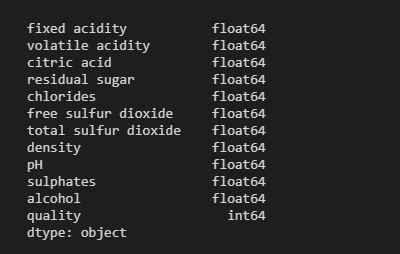
\includegraphics[width=0.8\textwidth]{image/type.png}
\caption{Typ danych znajdujących się w bazie.}
\end{figure}
\newpage
\textbf Klasyfikacji dokonałam na kolumnie \emph{quality}. Dane znajdujące się w tej kolumnie są liczbami całkowitymi.

\begin{figure}[!htb]
\centering
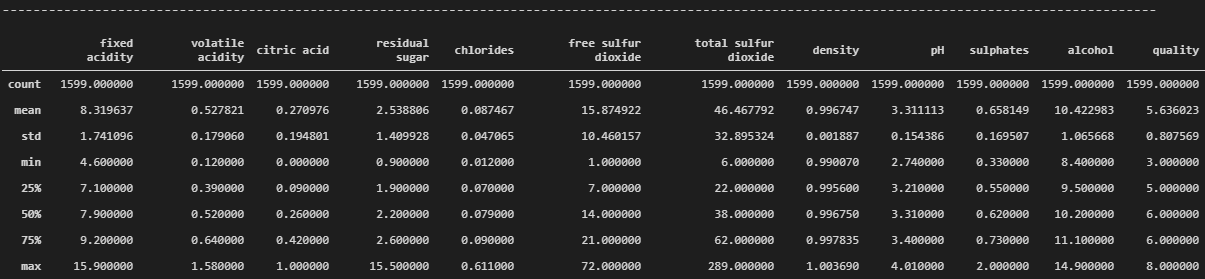
\includegraphics[width=0.8\textwidth]{image/mix.png}
\caption{Min, max, średnia i
częstość występowania poszczególnych odpowiedzi.}
\end{figure}

\begin{figure}[!htb]
\centering
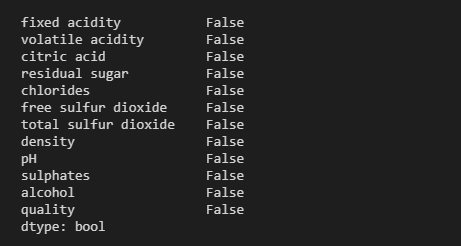
\includegraphics[width=0.8\textwidth]{image/data.png}
\caption{Baza w żaden sposób nie została zmodyfikowana, wszystkie dane były kompletne..}
\end{figure}

\section{Porównanie poznanych klasyfikatorów}

\subsection{Zestaw testowy i treningowy}

\begin{python}
print ('Zestaw treningowy:', X_train.shape,  y_train.shape)
print ('Zestaw testowy:', X_test.shape,  y_test.shape)
\end{python}

\begin{figure}[!htb]
\centering
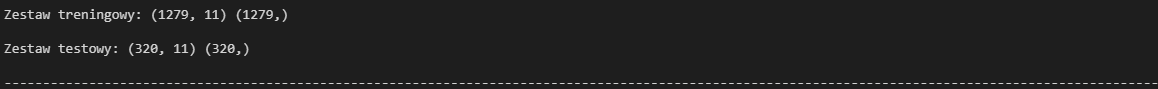
\includegraphics[width=0.8\textwidth]{image/zestaw.png}
\end{figure}

\section{Testowanie klasyfikatorów}

\subsection{k Najbliższych sąsiadów (dla wybranego k)}
\textbf{k - algorytm najbliższych sąsiadów} \emph{(ang. k - nearest neighbours, k-NN)}:
\begin{itemize}
\item[*] prosty klasyfikator (ściślej: algorytm regresji nieparametrycznej używany w statystyce do prognozowania wartości pewnej zmiennej losowej)
\item[*] klasyfikacja nowych przypadków jest realizowana na
bieżąco, tj. gdy pojawia się potrzeba klasyfikacji nowego
przypadku
\end{itemize}

\subsubsection{k Najbliższych sąsiadów (dla k = 6)}

\begin{figure}[!htb]
\centering
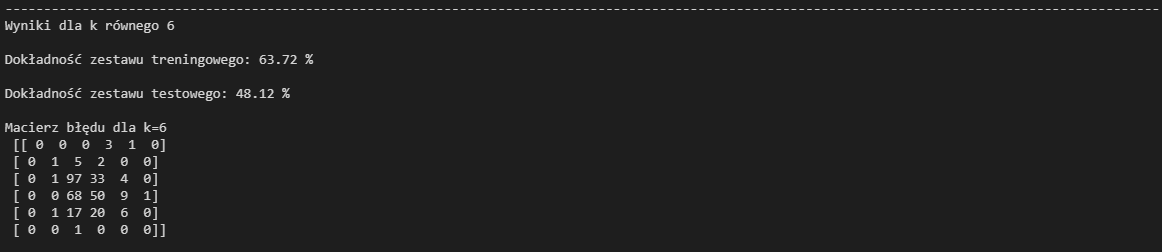
\includegraphics[width=\textwidth]{image/k_6.png}
\caption{Macierz błędu, dokładność zestawu testowego i treningowego.}
\end{figure}

\begin{figure}[!htb]
\centering
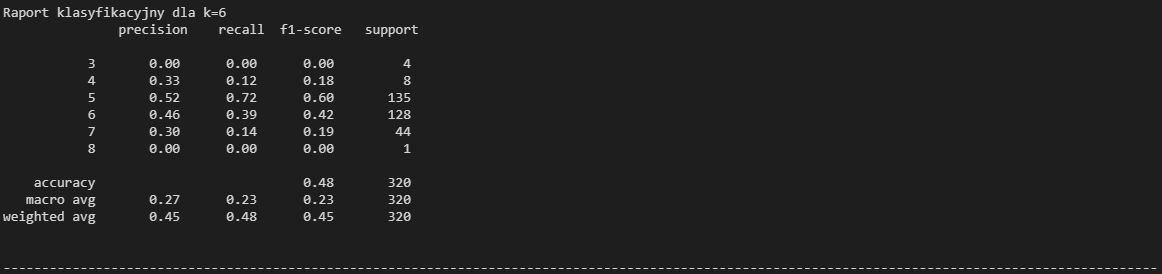
\includegraphics[width=\textwidth]{image/k_6_raport.png}
\caption{Raport klasyfikacyjny dla k równego 6.}
\end{figure}
\newpage
\subsubsection{k Najbliższych sąsiadów (dla k = 5)}

\begin{figure}[!htb]
\centering
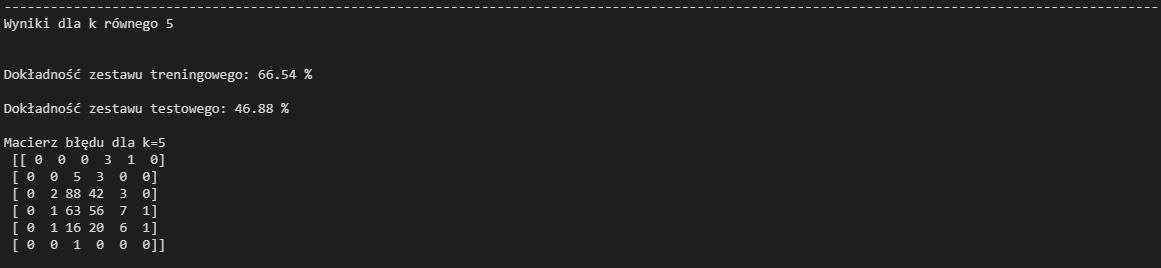
\includegraphics[width=\textwidth]{image/k_5.png}
\caption{Macierz błędu, dokładność zestawu testowego i treningowego.}
\end{figure}

\begin{figure}[!htb]
\centering
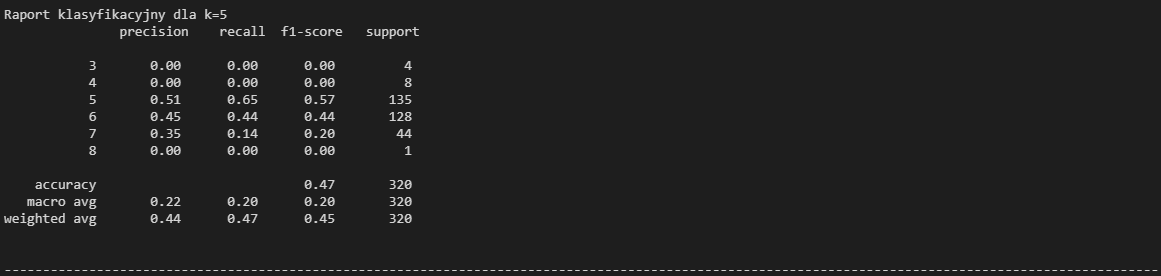
\includegraphics[width=\textwidth]{image/raport_k5.png}
\caption{Raport klasyfikacyjny dla k równego 5.}
\end{figure}

\subsubsection{k Najbliższych sąsiadów (dla k = 2)}

\begin{figure}[!htb]
\centering
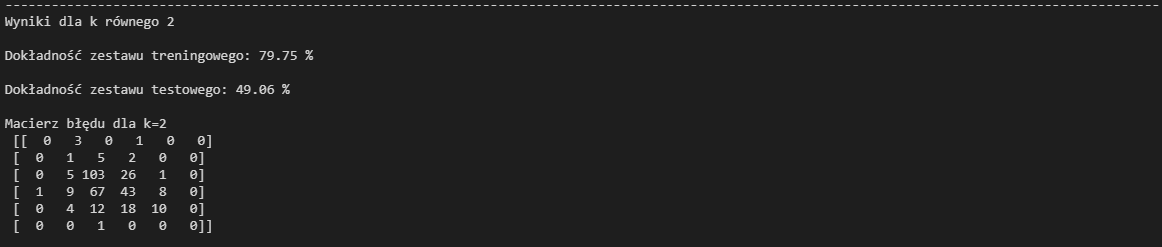
\includegraphics[width=\textwidth]{image/k_2.png}
\caption{Macierz błędu, dokładność zestawu testowego i treningowego.}
\end{figure}

\begin{figure}[!htb]
\centering
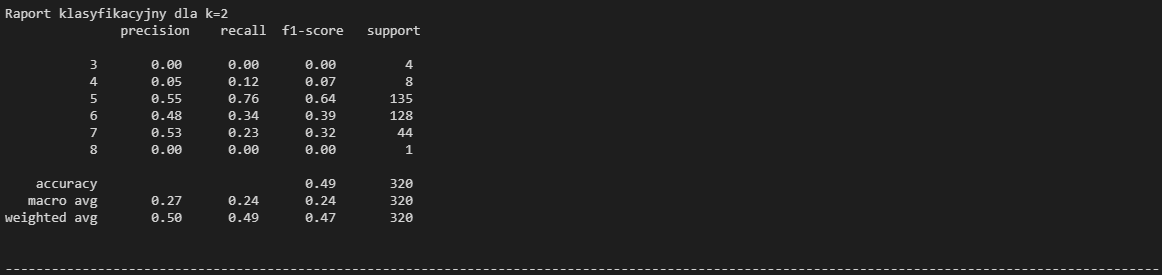
\includegraphics[width=\textwidth]{image/raport_k_2.png}
\caption{Raport klasyfikacyjny dla k równego 2.}
\end{figure}
\newpage
\subsubsection{k Najbliższych sąsiadów (dla k = 1)}

\begin{figure}[!htb]
\centering
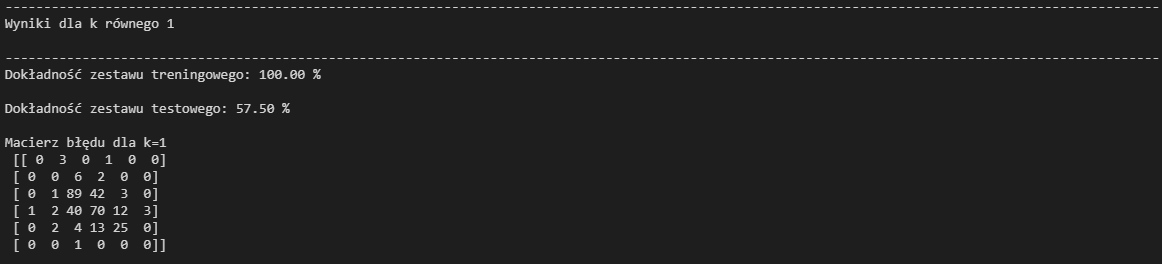
\includegraphics[width=\textwidth]{image/k_1.png}
\caption{Macierz błędu, dokładność zestawu testowego i treningowego.}
\end{figure}

\begin{figure}[!htb]
\centering
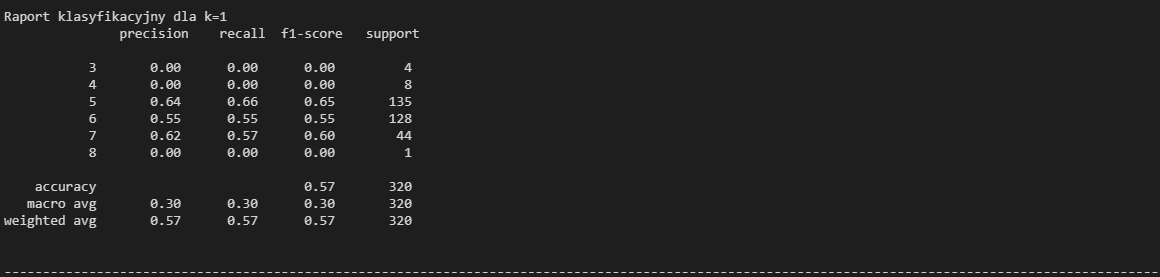
\includegraphics[width=\textwidth]{image/raport_k_1.png}
\caption{Raport klasyfikacyjny dla k równego 1.}
\end{figure}

\subsection{Naive Bayes}

\textbf{Naiwny klasyfikator bayesowski} \emph{(ang. Naive Bayes)} - prosty klasyfikator probabilistyczny. Naiwne klasyfikatory bayesowskie są oparte na założeniu o wzajemnej niezależności predyktorów (zmiennych niezależnych). Często nie mają one żadnego związku z rzeczywistością i właśnie z tego powodu nazywa się je naiwnymi. Bardziej opisowe jest określenie – „model cech niezależnych”. Ponadto model prawdopodobieństwa można wyprowadzić korzystając z twierdzenia Bayesa.

W zależności od rodzaju dokładności modelu prawdopodobieństwa, naiwne klasyfikatory bayesowskie można skutecznie „uczyć” w trybie uczenia z nadzorem. W wielu praktycznych aplikacjach, estymacja parametru dla naiwnych modeli Bayesa używa metody maksymalnego prawdopodobieństwa a posteriori; inaczej mówiąc, można pracować z naiwnym modelem Bayesa bez wierzenia w twierdzenie Bayesa albo używania jakichś metod Bayesa.
\newpage
\begin{figure}[!htb]
\centering
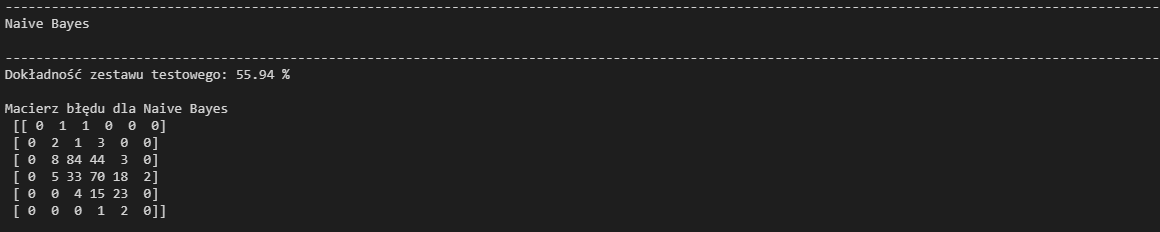
\includegraphics[width=\textwidth]{image/NV.png}
\caption{Macierz błędu, dokładność zestawu testowego i treningowego.}
\end{figure}

\begin{figure}[!htb]
\centering
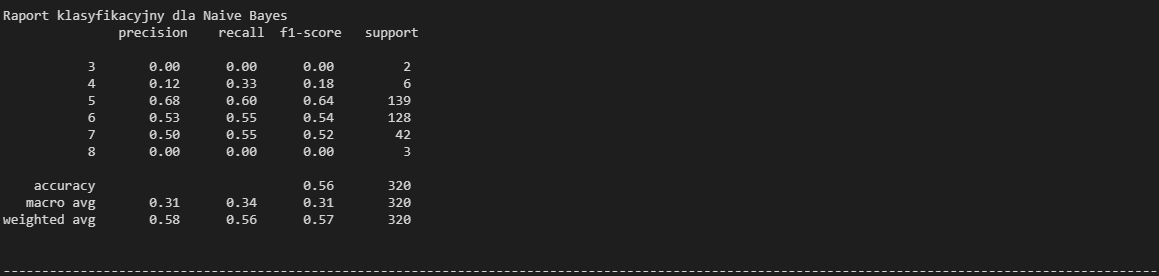
\includegraphics[width=\textwidth]{image/raport_NV.png}
\caption{Raport klasyfikacyjny dla Naive Bayes.}
\end{figure}

\subsection{Drzewa decyzyjne}

\textbf{Drzewa decyzyjne} \emph{(ang. Decision Tree)} - drzewa decyzyjne znajdują praktyczne zastosowanie w różnego rodzaju problemach
decyzyjnych, szczególnie takich gdzie występuje dużo rozgałęziających się wariantów a także
w warunkach ryzyka. Wiele algorytmów uczenia się wykorzystuje drzewa decyzyjne do
reprezentacji hipotez. Zgodnie z ogólnym celem uczenia się indukcyjnego, dążą one do
uzyskania drzewa decyzyjnego klasyfikującego przykłady trenujące z niewielkim błędem
próbki i o możliwie niewielkim rozmiarze, w nadziei, że takie drzewo będzie miało również
niewielki błąd rzeczywisty. Drzewa decyzyjne znajdują szerokie zastosowanie w problemach
związanych z klasyfikacją i predykcją pojęć typu: 

\begin{itemize}
\item[*] diagnostyka medyczna, 
\item[*] przewidywanie wydajności, 
\item[*] i wiele więcej 
\end{itemize}
\textbf{} Proces klasyfikacji z wykorzystaniem drzew decyzyjnych jest efektywny obliczeniowo,
wyznaczenie kategorii przykładu wymaga w najgorszym razie przetestowania raz wszystkich
jego atrybutów. 
\newpage
\begin{figure}[!htb]
\centering
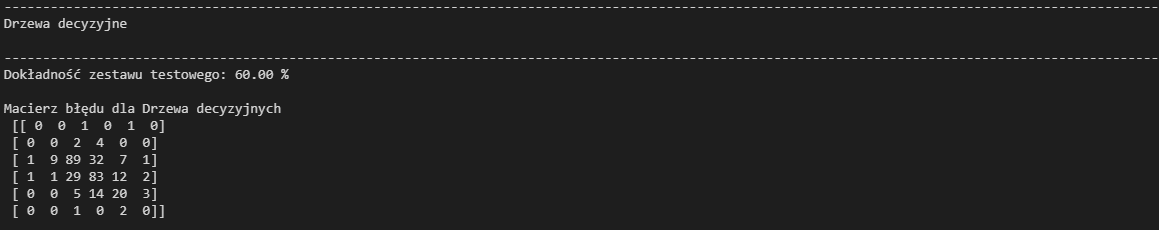
\includegraphics[width=\textwidth]{image/DD.png}
\caption{Macierz błędu, dokładność zestawu testowego i treningowego.}
\end{figure}

\begin{figure}[!htb]
\centering
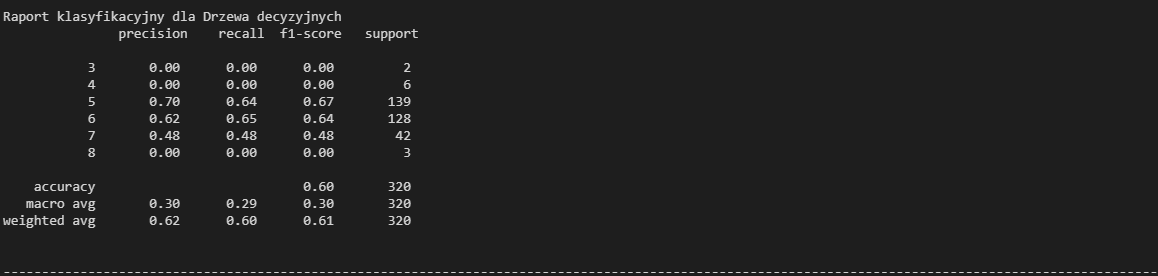
\includegraphics[width=\textwidth]{image/raport_DD.png}
\caption{Raport klasyfikacyjny dla Drzew decyzyjnych.}
\end{figure}

\subsection{Random Forest}

\textbf{Las losowy} \emph{(ang. Random forest)} - lub losowy las decyzyjny (Random decision forest) – metoda zespołowa uczenia maszynowego dla klasyfikacji, regresji i innych zadań, która polega na konstruowaniu wielu drzew decyzyjnych w czasie uczenia i generowaniu klasy, która jest dominantą klas (klasyfikacja) lub przewidywaną średnią (regresja) poszczególnych drzew. Losowe lasy decyzyjne poprawiają tendencję drzew decyzyjnych do nadmiernego dopasowywania się do zestawu treningowego. Pierwszy algorytm losowych lasów decyzyjnych został stworzony przez Tina Kam Ho przy użyciu metody losowej podprzestrzeni, która w formule Ho jest sposobem na implementację podejścia „dyskryminacji stochastycznej” do klasyfikacji zaproponowanej przez Eugene'a Kleinberga.

\begin{figure}[!htb]
\centering
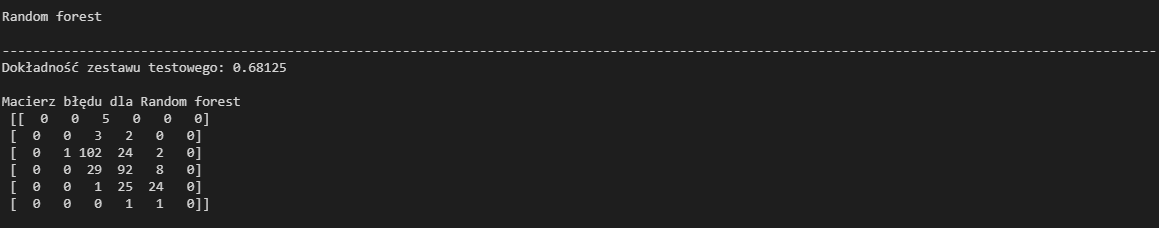
\includegraphics[width=\textwidth]{image/RF.png}
\caption{Macierz błędu, dokładność zestawu testowego i treningowego.}
\end{figure}
\newpage
\begin{figure}[!htb]
\centering
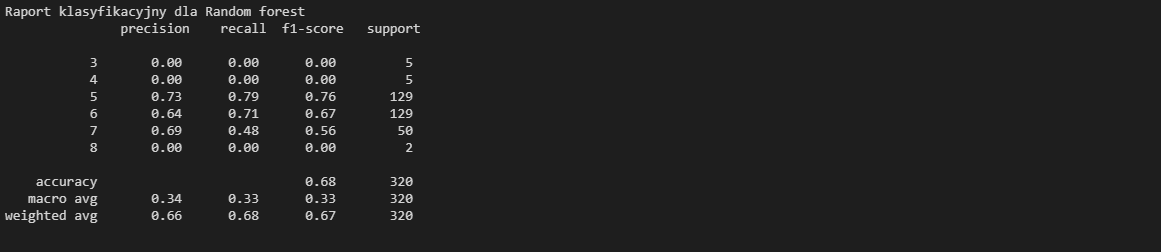
\includegraphics[width=\textwidth]{image/repo_RF.png}
\caption{Raport klasyfikacyjny dla Random Forest.}
\end{figure}

\subsection{Support Vector Machines}

\textbf{Maszyna wektorów nośnych, maszyna wektorów podpierających} \emph{(ang. Support Vector Machine, SVM)} - abstrakcyjny koncept maszyny, która działa jak klasyfikator, a której nauka ma na celu wyznaczenie hiperpłaszczyzny rozdzielającej z maksymalnym marginesem przykłady należące do dwóch klas. Często wykorzystywana niejawnie w procesie rozpoznawania obrazów. Maszyna wektorów nośnych, korzystająca z jądra RBF jest w stanie klasyfikować nierozdzielne liniowo klasy. W przypadku, wystąpienia więcej niż jednej klasy maszynę wektorów nośnych zazwyczaj uczy się metodą OvR.

\begin{figure}[!htb]
\centering
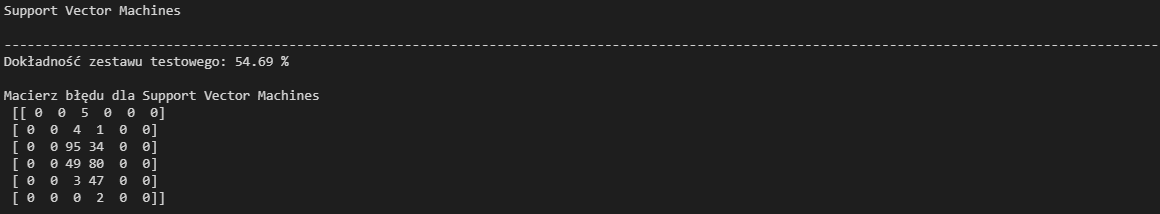
\includegraphics[width=\textwidth]{image/SVM.png}
\caption{Macierz błędu, dokładność zestawu testowego i treningowego.}
\end{figure}

\begin{figure}[!htb]
\centering
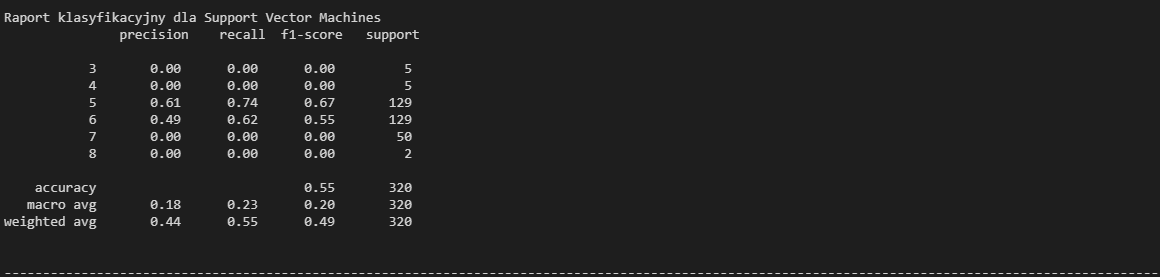
\includegraphics[width=\textwidth]{image/raport_SVM.png}
\caption{Raport klasyfikacyjny dla Support Vector Machines.}
\end{figure}
\newpage
\subsection{Sieci neuronowe}

\textbf{Sieć neuronowa} \emph{(ang. Neural Network)} - ogólna nazwa struktur matematycznych i ich programowych lub sprzętowych modeli, realizujących obliczenia lub przetwarzanie sygnałów poprzez rzędy elementów przetwarzających, zwanych sztucznymi neuronami, wykonujących pewną podstawową operację na swoim wejściu. Oryginalną inspiracją takiej struktury była budowa naturalnych neuronów, łączących je synaps, oraz układów nerwowych, w szczególności mózgu.

Czasem nazwą „sztuczne sieci neuronowe” określa się interdyscyplinarną dziedzinę wiedzy zajmującą się konstrukcją, trenowaniem i badaniem możliwości tego rodzaju sieci.

\begin{figure}[!htb]
\centering
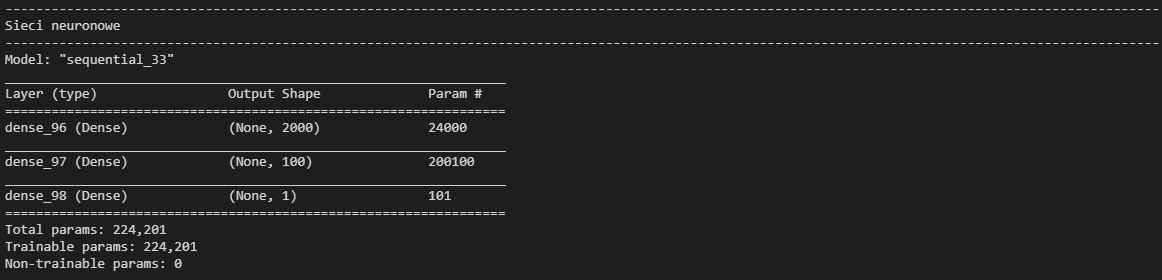
\includegraphics[width=\textwidth]{image/SN1.png}
\caption{Sieci neuronowe}
\end{figure}

\begin{figure}[!htb]
\centering
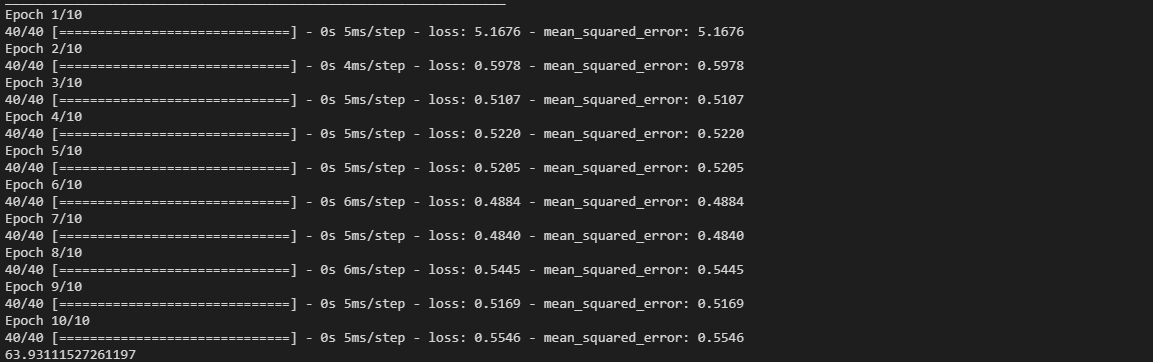
\includegraphics[width=\textwidth]{image/SN2.png}
\caption{Ocena dla modelu losowego.}
\end{figure}

\begin{figure}[!htb]
\centering
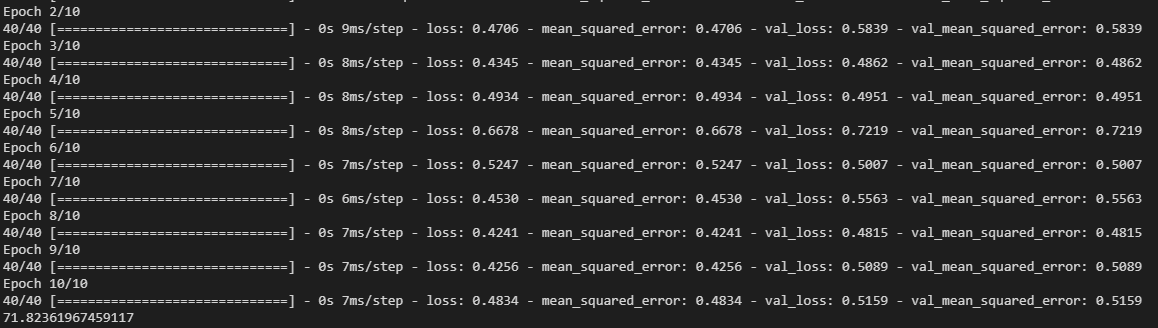
\includegraphics[width=\textwidth]{image/SN3.png}
\caption{Ocena modelu sieci neuronowej.}
\end{figure}

\newpage

\section{Podsumowanie}
\textbf{} Najlepsze wyniki otrzymałam za pomocą klasyfikatorów: \emph{Random Forest, dokładność to \emph{71.56\%}}. Na drugim miejscu znalazły się \emph{Sieci neuronowe, dokładność to \emph{66.46\%}}.

\newpage
\section{Reguły asocjacyjne}

\subsubsection{Co to są reguły asocjacyjne?}
Reguły asocjacyjne przypominają reguły decyzyjne omawiane na poprzednim wykładzie. Tym razem jednak decyzja (prawa strona implikacji) nie jest z góry określona, tzn. nie wiemy, na którym atrybucie ma się opierać. Jest to przykład nauki bez nauczyciela (podobnie, jak w przypadku algorytmów grupowania): algorytm nie ma określonej z góry prawidłowej odpowiedzi, zamiast tego ma opisać wewnętrzne zależności między atrybutami.

\subsubsection{Czy szukanie reguły asocjacyjnych ma sens?}
Wyszukiwanie reguł asocjacyjnych ma za zadanie zwiększyć wydajność systemów baz danych pod względem funkcjonalności umożliwiając zadawanie złożonych zapytań przykładowo w posta- ci: Znajdź wszystkie reguły, których konsekwencją jest sprzedaż produktu \emph{X}. Znajomość reguł tego typu pozwoli podnieść sprzedaż produktu \emph{X}.

\subsubsection{Rodzaje reguł asosjacyjnych}
\begin{itemize}
\item[*] jednowymiarowe, 
\item[*] wielowymiarowe, 
\end{itemize}
\section{Porównywanie klasyfikatorów na wykresie}
\begin{figure}[!htb]
\centering
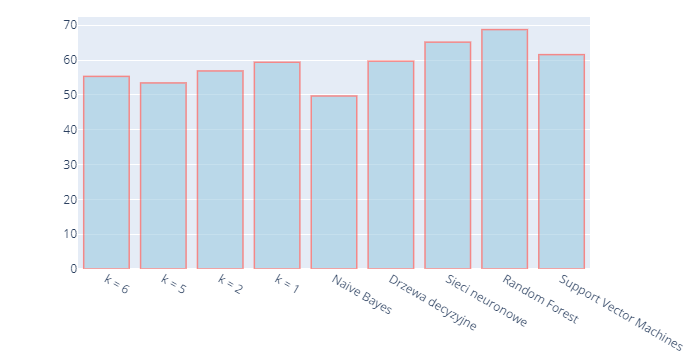
\includegraphics[width=\textwidth]{image/wykres.png}
\caption{Porównywanie klasyfikatorów na podstawie oceny modelu.}
\end{figure}

\end{document}